\documentclass[12pt]{article}

\usepackage[utf8]{inputenc}
\usepackage[T1]{fontenc}
\usepackage{lmodern}
\usepackage{geometry}
\usepackage{xcolor}
\usepackage{tikz}
\usepackage{booktabs}
\usepackage{enumitem}
\usepackage{hyperref}
\usepackage{fancyhdr}
\usepackage{titlesec}
\usepackage{parskip}

\geometry{margin=1.25in, top=1in, bottom=1in}

% Colors
\definecolor{accent}{RGB}{41, 128, 185}
\definecolor{success}{RGB}{39, 174, 96}
\definecolor{warning}{RGB}{243, 156, 18}
\definecolor{danger}{RGB}{192, 57, 43}
\definecolor{lightgray}{RGB}{245, 245, 245}

% Section styling
\titleformat{\section}{\Large\bfseries\color{accent}}{}{0em}{}[\titlerule]
\titleformat{\subsection}{\large\bfseries}{}{0em}{}
\titlespacing*{\section}{0pt}{2em}{1em}
\titlespacing*{\subsection}{0pt}{1.5em}{0.5em}

% Header/Footer
\pagestyle{fancy}
\fancyhf{}
\rhead{\textcolor{gray}{FAST15M System}}
\lhead{\textcolor{gray}{Technical Overview}}
\rfoot{\textcolor{gray}{\thepage}}
\renewcommand{\headrulewidth}{0.4pt}

\hypersetup{
    colorlinks=true,
    linkcolor=accent,
    urlcolor=accent
}

\begin{document}

% Title Page
\begin{titlepage}
\centering
\vspace*{2cm}

{\Huge\bfseries\color{accent} FAST15M}\\[0.5cm]
{\Large Latency Arbitrage on Polymarket}\\[2cm]

{\large A system that trades 15-minute crypto prediction markets\\by reacting to price changes faster than the market adjusts.}

\vfill


\begin{tikzpicture}
\draw[accent, line width=2pt] (0,0) -- (12,0);
\end{tikzpicture}

\vspace{1cm}
{\large January 2026}\\[0.5cm]
{\small Technical Overview for General Audience}

\end{titlepage}

%==============================================================================
\section{The Big Picture}
%==============================================================================

\textbf{What we're trading:} Polymarket offers simple yes/no bets on whether Bitcoin (and other cryptos) will go up or down in the next 15 minutes.

\textbf{The opportunity:} When Bitcoin's price moves on Binance (the world's largest crypto exchange), it takes time for Polymarket's betting odds to catch up. We try to place bets during that window.

\textbf{The edge:} If we can consistently predict the outcome slightly better than the current odds suggest, and bet the right amount, we make money over time.

\vspace{1em}
\begin{center}
\begin{tikzpicture}[
    box/.style={draw, rounded corners, minimum width=3cm, minimum height=1cm, align=center},
    arrow/.style={->, thick, >=stealth}
]
    \node[box, fill=blue!10] (binance) at (0,0) {Binance\\Price Moves};
    \node[box, fill=yellow!20] (window) at (5,0) {Time Window\\(our opportunity)};
    \node[box, fill=green!10] (poly) at (10,0) {Polymarket\\Odds Adjust};
    
    \draw[arrow] (binance) -- (window);
    \draw[arrow] (window) -- (poly);
    
    \node[below=0.3cm of window, text width=4cm, align=center, font=\small] {We place bets here};
\end{tikzpicture}
\end{center}

%==============================================================================
\section{How It Works (Step by Step)}
%==============================================================================

\subsection{Step 1: Watch Binance Prices}

We connect directly to Binance's data feed and receive price updates for BTC, ETH, SOL, and XRP. Our system processes these updates extremely fast:

\begin{center}
\colorbox{lightgray}{
\begin{minipage}{0.8\textwidth}
\vspace{0.5em}
\textbf{Measured Performance}\\[0.5em]
Time to process each price update: \textbf{15--80 microseconds}\\
{\small (A microsecond is one millionth of a second)}\\[0.5em]
\textit{Source: FeedMetrics instrumentation in our codebase}
\vspace{0.5em}
\end{minipage}
}
\end{center}

\subsection{Step 2: Calculate the ``True'' Probability}

When the price moves, we calculate what we think the real probability of ``Up'' is. 

\textbf{Simple example:} If Bitcoin has gone up 0.5\% with 10 minutes left, and it's been moving around a lot (high volatility), there's maybe a 60\% chance it stays up. If it's been calm (low volatility), maybe 75\%.

We use a mathematical model (``driftless lognormal'') that accounts for:
\begin{itemize}[nosep]
    \item How much the price has already moved
    \item How volatile the asset has been recently
    \item How much time is left in the 15-minute window
\end{itemize}

\subsection{Step 3: Compare to Market Odds}

Polymarket shows prices like ``Up: \$0.55'' --- meaning the market thinks there's a 55\% chance of Up.

If our model says 65\% but the market says 55\%, we have a potential \textbf{10\% edge}.

\subsection{Step 4: Decide How Much to Bet}

We don't bet our whole bankroll. We use the ``Kelly Criterion'' --- a formula that tells you the optimal bet size based on your edge and the odds.

\begin{center}
\colorbox{lightgray}{
\begin{minipage}{0.8\textwidth}
\vspace{0.5em}
\textbf{Our Betting Rules}\\[0.5em]
$\bullet$ Never bet more than 1\% of bankroll on one trade\\
$\bullet$ Only bet if our edge is at least 1\%\\
$\bullet$ Use ``quarter Kelly'' (bet 1/4 of theoretically optimal) for safety\\[0.5em]
\textit{Source: kelly.rs and updown15m.rs in our codebase}
\vspace{0.5em}
\end{minipage}
}
\end{center}

\subsection{Step 5: Execute the Trade}

If all conditions are met, we send an order to Polymarket.

\begin{center}
\colorbox{lightgray}{
\begin{minipage}{0.8\textwidth}
\vspace{0.5em}
\textbf{Measured Speed (Internal Processing)}\\[0.5em]
From price update to order decision: \textbf{under 1 millisecond}\\
{\small (This does NOT include the time to actually send to Polymarket)}\\[0.5em]
\textit{Source: TradeSpan instrumentation in fast15m\_reactive.rs}
\vspace{0.5em}
\end{minipage}
}
\end{center}

%==============================================================================
\section{What We've Actually Measured}
%==============================================================================

It's important to separate what we \textit{know} from what we \textit{believe}.

\vspace{1em}
\begin{center}
\renewcommand{\arraystretch}{1.4}
\begin{tabular}{p{6cm}cc}
\toprule
\textbf{What} & \textbf{Status} & \textbf{Value} \\
\midrule
Time to decode Binance messages & \textcolor{success}{Measured} & 15--80 $\mu$s \\
Internal decision time & \textcolor{success}{Measured} & $<$1 ms \\
Time for data to travel from Binance & \textcolor{warning}{Estimated} & 8--30 ms \\
Time for orders to reach Polymarket & \textcolor{danger}{Unknown} & ??? \\
Actual fill rate on orders & \textcolor{danger}{Unknown} & ??? \\
Whether we're faster than others & \textcolor{danger}{Unknown} & ??? \\
\bottomrule
\end{tabular}
\end{center}

\vspace{1em}
\textbf{Legend:} 
\textcolor{success}{$\bullet$ Measured} = We have real data from our system.
\textcolor{warning}{$\bullet$ Estimated} = Calculated, but with uncertainty.
\textcolor{danger}{$\bullet$ Unknown} = We haven't done live trading yet.

%==============================================================================
\section{The Hypothesis (What We Believe)}
%==============================================================================

Our core belief is:

\begin{quote}
\textit{``When Binance prices move, there's a brief window (maybe 500ms to 2 seconds) before Polymarket odds fully adjust. If we can place bets during that window, we capture the edge.''}
\end{quote}

\textbf{This is not yet proven.} We've built the system to test this hypothesis. Here's what needs to happen:

\vspace{0.5em}
\begin{enumerate}[nosep]
    \item \textbf{Validate the window exists:} Measure the actual time lag between Binance moves and Polymarket adjustments.
    \item \textbf{Measure execution speed:} Find out how long it really takes to get orders filled on Polymarket.
    \item \textbf{Check fill rates:} See if our orders actually execute, or if the opportunity disappears before we can act.
    \item \textbf{Track profitability:} After fees and slippage, do we actually make money?
\end{enumerate}

%==============================================================================
\section{Why It Might Work}
%==============================================================================

\subsection{The Market Structure Favors Speed}

\begin{itemize}[nosep]
    \item 15-minute windows are short --- not much time for prices to ``mean revert''
    \item Binary outcomes (Up or Down) are simple --- no complex hedging needed
    \item Polymarket uses an orderbook (first-come-first-served) --- speed matters
\end{itemize}

\subsection{Our Technical Implementation}

\begin{itemize}[nosep]
    \item \textbf{Fast data processing:} We use specialized libraries (simd-json) that parse data 10--50x faster than standard methods
    \item \textbf{No waiting:} Our system reacts to every price change instantly, not on a timer
    \item \textbf{Smart caching:} We keep Polymarket orderbook data ready so we don't have to fetch it when making decisions
\end{itemize}

\subsection{Conservative Risk Management}

\begin{itemize}[nosep]
    \item We deliberately underestimate our edge (``shrink toward 50\%'')
    \item We bet small (1\% max per trade)
    \item We diversify across 4 assets
\end{itemize}

%==============================================================================
\section{Why It Might Not Work}
%==============================================================================

We're honest about the risks:

\vspace{0.5em}
\textbf{1. The window might not exist (or be too small)}

Maybe Polymarket market makers are already watching Binance and adjust instantly. We won't know until we try.

\vspace{0.5em}
\textbf{2. Execution might be too slow}

Even if we decide fast, getting orders to Polymarket and filled might take too long. The opportunity could vanish.

\vspace{0.5em}
\textbf{3. Adverse selection}

Maybe our orders only get filled when we're \textit{wrong} --- smart market makers pull their quotes when they see the price moving against them.

\vspace{0.5em}
\textbf{4. Model error}

Our probability model assumes prices move smoothly. In reality, they can jump. Our 65\% estimate might actually be 50\%.

\vspace{0.5em}
\textbf{5. Competition}

If others are doing the same thing faster, we lose.

%==============================================================================
\section{Current Status}
%==============================================================================

\begin{center}
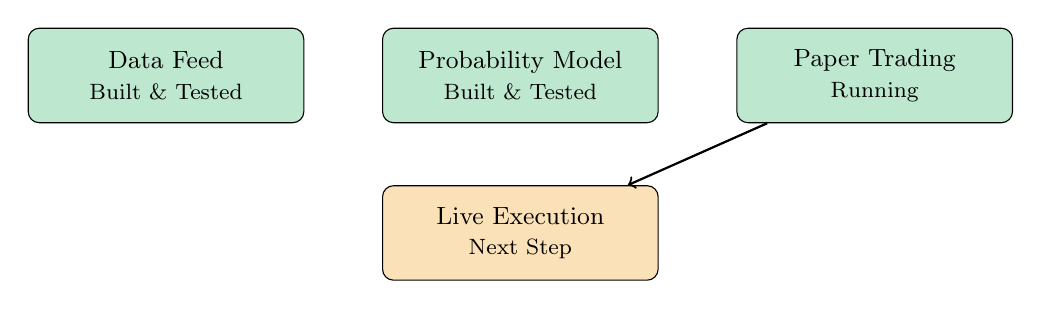
\begin{tikzpicture}[
    box/.style={draw, rounded corners, minimum width=3.5cm, minimum height=1.2cm, align=center, font=\small},
]
    \node[box, fill=success!30] (done1) at (0,0) {Data Feed\\{\footnotesize Built \& Tested}};
    \node[box, fill=success!30] (done2) at (4.5,0) {Probability Model\\{\footnotesize Built \& Tested}};
    \node[box, fill=success!30] (done3) at (9,0) {Paper Trading\\{\footnotesize Running}};
    
    \node[box, fill=warning!30] (next) at (4.5,-2) {Live Execution\\{\footnotesize Next Step}};
    
    \draw[->, thick] (done3) -- (next);
\end{tikzpicture}
\end{center}

\textbf{What's done:}
\begin{itemize}[nosep]
    \item Binance data feed with sub-millisecond processing
    \item Probability model with volatility estimation
    \item Position sizing with Kelly criterion
    \item Paper trading simulation
    \item Full instrumentation to measure everything
\end{itemize}

\textbf{What's next:}
\begin{itemize}[nosep]
    \item Connect to Polymarket for real order execution
    \item Measure actual fill rates and latency
    \item Validate (or disprove) the hypothesis with real money
\end{itemize}

%==============================================================================
\section{Bottom Line}
%==============================================================================

\begin{center}
\colorbox{lightgray}{
\begin{minipage}{0.85\textwidth}
\vspace{0.5em}
\textbf{FAST15M is a bet on a simple idea:}\\[0.5em]
Information takes time to flow from Binance to Polymarket. If we can act in that window, we can profit.\\[0.5em]
We've built the infrastructure to test this. The technical foundation is solid (measured sub-millisecond internal latency). What remains is live validation.\\[0.5em]
\textbf{The question isn't ``does our code work?'' --- it does.}\\
\textbf{The question is ``does the edge exist and can we capture it?''}\\[0.5em]
Only live trading will tell.
\vspace{0.5em}
\end{minipage}
}
\end{center}

\vfill
\begin{center}
\textcolor{gray}{\small Document generated January 2026 $\bullet$ All latency measurements from production codebase instrumentation}
\end{center}

\end{document}
